\chapter{User Study of The TP Community}
\label{ChapterWorkshop}
The tasks presented in \autoref{TaskAndMethods} serve as proposals for how to include the users as an active part of the design process at TC Electronic in correlation with developing a platform for sharing User TonePrints. The tasks are all considered equally important, but ultimately only one of them is explored in this project due to the restricted timeframe. Through discussions with our company supervisor, task 1 is chosen for this purpose. The following chapter will start with an elaboration on this decision before moving on to the execution and subsequent analysis of the results, including what methods are applied for both parts.

\section{Deciding on a task}
\label{TaskDecision}
As described in \autoref{Task1}, the purpose of task 1 is to investigate how to design the information architecture of the TonePrint community, in order to ensure that the design accommodates to the users' mental model of the system. Many considerations were put in to the decision of conducting this task, including TC's wishes, how well it would fit into a typical SCRUM sprint, the remaining timeframe for this project etc. The impact of all these factors also influenced what methods to consider and how to approach them.

Firstly, an investigation of the information architecture seemed the most fitting to conduct due to the current state of the TonePrint community. TC are at a very early stage of development, as no version of a sharing platform currently exist. TC therefore considered it evident to start with an assessment of how content and features should be structured as a baseline for the future design process.

Secondly, previous investigations in this project have showed how TC follows the SCRUM framework in the shape of 3-week sprints (see \autoref{ThemanticAnalysis}). As such, much of the discussion was on finding a task and suitable method that could easily fit to this timeframe, and task 1 was here considered ideal. the limited time remaining on the project furthermore required to conduct it as a 2-week sprint, and even though this is not the same duration as a sprint at TC, conducting a task in this timeframe will still provide insight into how UX tests can fit to a short time period. Task 3 and 4 could just as well fit this timeframe, but each of them require an existing app to some extend. It wouldn't necessarily have to be a fully functional system, but still one that could represent the appearance and functionalities of the system.

Thirdly, task 5 focusing on creating personas of the typical users of TC products was considered very valuable for TC in their understanding of them. However, this task is too extensive and time-consuming to execute in a 2-week sprint and is in general considered a semester project on its own. If it were to be executed anyway, it would only result in demographical info on the users, which doesn't provide anything new for TC.\\

\noindent
When choosing task 1, further specifying the approach is required, as it proposes two different ones. One of these is through Lo-fi testing which is a great tool, but as it is elaborated on in \autoref{Task1}, it requires a rough idea of how the system should work and how the information should be presented. For the TonePrint community there currently is no rough idea of how it should look, and it would as such make more sense to include the users in shaping the concept and flow of the community from the bottom through a \textit{participatory design procedure}. The approach should then follow the outlined suggestion in \autoref{Task1} by conducting a workshop with potential end-users as subjects in order to explore their mental models of a TonePrint community. \fxnote{Research question?}

\section{Mental Models}
\label{MentalModel}
Before proposing the experimental design and setup of a workshop, it seems appropriate to first define what is meant by \textit{mental models}, and how they are constructed. In \autoref{UXbenefits} it is mentioned that if the developers have the same understanding of how a given product should look and behave, then the users are more likely to have a pleasant experience. Other factors such as the users' hedonic opinions of the product also play a role, but this was also meant as a quick introduction to the term. In general, mental models are types of conceptual models that resides in people minds, as the name implies. In other words, mental models are the users' understanding of how something works. The definition of a conceptual model is already outlined in \autoref{CommunityConcept} as an explanation of how something works, including all concepts in it, and how they relate to each other. For mental models, different people may hold different versions for the same system, and some people may even hold multiple models of the same system, focusing on different aspects of its operation \parencite[][26]{PDF:DonNorman}. \\

\noindent
When it comes to constructing mental models, \textcite{PDF:MentalModelInstructions} defines three different factors that influence this process. These are the individuals ability to utilise existing models that relate to the matter in question, general observations of the outside world, and explanations from other people \parencite[][68-69]{PDF:MentalModelInstructions}. It should be noted that the "existing models" can be both internal and external models of similar systems, as long as they can serve as analogies for the model to be created. When this is put into context with the TonePrint community, it is as such expected that the users will construct mental models on the basis of:
%
\begin{itemize}
	\item Their understanding of how the current TonePrint app works, including TC's influence on this understanding.
	\item Observations of how other users utilise the TonePrint app and currently attempt to share User TonePrints with each other.
	\item What other end-users i.e. guitarists tell them.
\end{itemize}
%
A proper mental model allows the user to predict the outcome of possible actions, even if these actions haven't occurred. In such cases, the cognitive system replaces the stimulus in question with inputs from the mental model, interprets them, and draws a conclusion, further strengthening the mental model for future scenarios \parencite[][64]{PDF:MentalModelInstructions}. For task 1, it's important to remember that the main goal for uncovering mental models is to do so in correlation with assessing how the information architecture should be shaped. \autoref{Task1} already proposes examples of how this could be approached in short, and a further elaboration is therefore required, which will be provided in the following section.

\section{Experimental design}
\label{ExperimentalDesign}
Shaping the information architecture of a system requires multiple steps of generating ideas for content and communicating these, before moving on to testing them with the users \parencite[][356-364]{PDF:InformationArchitecture}. For this task, the first step would as such be to generate ideas for content and features to be included in the TonePrint community, and how they should communicate with each other? Instead of engaging in a phase of generating such ideas, this paper instead suggests to make use of studies already conducted by TC, focusing on the TonePrint community. A study by our company supervisor \textcite{PDF:BrugerWorkshopUserTonePrints}, investigates what is required from such a platform, and the result is given in the shape of a list of content which, if included, would make end-users more interested in using the platform \parencite[][35]{PDF:BrugerWorkshopUserTonePrints}. It's important to note that this content also is produced by the users in a workshop, and by utilizing this information, it will serve as a good starting point. Furthermore, the interview conducted with members of the TC staff previously in this project may also contain suitable content for developing an appropriate strategy for the information architecture.

With the ideas generated, the next step is then to explore the content with the users involved, and a suitable way of approaching this is through the card sorting method. Donna Spencer describes this in her book as \textit{a fairly straightforward tool that helps the developers understand the people they are designing for} \parencite[][6]{WEB:DonnaSpencer}. The method involves users sorting a set of cards into piles of what they find similar either according to predetermined group names, or they can be told to describe the categories themselves after the sort. These are referred to as an \textit{open card sort} and a \textit{closed card sort} respectively. The method is most commonly used for organising, grouping, and labeling elements when the focus is on information architecture \parencite[][10]{WEB:DonnaSpencer}, but this doesn't mean that the information can be structured from this method alone. While card sorting is a great tool for finding out what information belongs together, it doesn't provide answers to how these groupings should interact with each other. Donna Spencer also elaborates that she typically dosen't employ the method on its own because of the just stated reasons and that further user involvement is required for investigating the information architecture \parencite[][15]{WEB:DonnaSpencer}.

Proceeding from the card sort therefore requires methods looking into how the users will put the groupings into context with each other. Methods applicable for this purpose could be \textit{interviews}, where the users are given clarifying questions, or a \textit{survey} could be sent out to reach more people. Ultimately, it is decided to take a more observational approach by having the users explain how to complete specific tasks within the TonePrint community. Before elaborating on how how to specifically adapt this and the card sort, another important factor should be addressed. The subjects have to consist of potential end-users, as they represent the mental models of the people who are likely to use a finished version of the system on a regular basis. As it was mentioned in \autoref{MentalModel}, constructing a mental model is influenced by a persons ability to utilise existing models, among other things. For a more appropriate mental model, the subjects should therefore have to consist of guitarists and bassists who have some level of experience with using the current TonePrint app.

\subsection{The card sorting method}
\label{CardSort}
With the overall scope in place, a deeper look into how the methods should be adapted is needed. Specifying how to employ the card sorting method is done in multiple steps \parencite[][8]{WEB:DonnaSpencer}, where the first is deciding on what is to be investigated. As this already is clarified, attention can be turned to the next step which focusses on fitting specific elements of the methods. Firstly, the question of whether to conduct an open or closed card sort has already been mentioned, and it really depends on how much information is wanted from it. Open card sorts are generally used more frequently, as they convey much more information than a closed card sort, where the group labels are predetermined \parencite[][82]{WEB:DonnaSpencer}. The open card sort is therefore chosen to not only allow people to group cards but also decide themselves, what label they should have.

The next element focusses on whether to conduct it face-to-face or remote. The two deciding factors here are the diversity of TC's customer base and the limited time for conducting the study. TC have already been established as a world-wide known company with customers ranging from Canada to Australia. As such, it is seen as a great opportunity to gather a more diverse collection of responses by conducting a remote card sort instead of only recruiting subjects geographically available. The limited time of two weeks further supported this idea as a remote study can handle itself if it is set up in a proper program. The obvious counter-argument here is that this limits the subjects to only engage in either the card sort or the subsequent workshop tasks, and while this is true, it's decided to still approach it this way. While the card sort takes care of itself, it is possible to run a workshop in-person with a group of end-users at the same time. The time-frame of the workshop is shortened, and as long as the subjects taking part in either the card sort or workshop all are end-user, the job in the future analysis and discussion of this project is to unify the results from the tests. The main concern would be that if the workshop doesn't use the card sort as a starting point, the subjects won't have the necessary tools to complete the tasks, but since they are end-users, they are expected to know the necessary concepts.

The next step before sending the remote card sort to the subjects is the obvious task of choosing content and finding the best way of reaching the correct subjects. As it has already been mentioned, the cards for the card sort are developed from a TC study \parencite{PDF:BrugerWorkshopUserTonePrints} and the interview with the four members of TC's development team (see \autoref{ThemanticAnalysis}), but before formulating them, some considerations should be made to the number of cards. By consulting Donna Spencer, the number should be somewhere between 30 and 100 cards, as fewer than 30 cards may make it difficult to create groups and more than 100 cards might make it too tiring to sort. Nielsen norman group also has opinions to this with a range limited to 40-80 cards \parencite{WEB:NielsenNormanCardSort}. 40 cards are ultimately formulated, each representing a piece of content for the TonePrint community, and during this phase it's important to formulate the content similarly enough to suggest potential groupings while not unnecessarily influencing the card sort. A common mistake when formulating cards is mixing content with functionality, however, in many cases it is possible to rephrase the cards so they are presented at a similar level \parencite[][103-107]{WEB:DonnaSpencer}. 

The card sort is sent to the users as a link in the Facebook group \textit{TonePrint junkies} consisting of more than 4000 TonePrint users around the world, hoping that it will produce some responses. It's however not alarming, should the number of responses be low. Donna Spencer argues that for studies trying to produce statistically valid conclusion, much attention should be given to recruiting the right amount of participants, but for studies focusing on information architecture this isn't particularly relevant \parencite[][130]{WEB:DonnaSpencer}. Nonetheless, as another motivation for taking part in the card sort, the users are informed that they also will take part in a draw for a free TonePrint pedal, by agreement with TC. This is done by providing their email in a short survey following the card sort, where they also get a chance to explain the reasoning behind their created groups, as a way of gathering some qualitative data from the card sort. This survey and the 40 cards are all located in appendix?? \fxnote{Smid cards i appendix + survey'en}

\subsection{Workshop approach}
\label{WorkshopApproach}
With the card sort and workshop completely separated, the general run-time of the workshop is substantially shortened, which should ease recruiting, as the subjects are needed for a shorter period of time. The desired outcome of the workshop is to elicit end-users' mental models of the TonePrint community, but this is not how it should be phrased to the subjects, as this definition is to broad and likely won't make much sense to the them. The mental models should be explored in correlation with the new content that is being added to the current TonePrint concept, and the phrasing should therefore focus on this new content, including how the subjects would want to engage with it. On the basis of the interview with the developers at TC (see \autoref{HeuristicEvaluation}), it's clear that the new content overall consists of sharing User TonePrints with other users and downloading User TonePrints made by others. What is included within this content is investigated with the card sort, but the workshop may also shed some light on this matter. Two tasks are subsequently formulated from this, and they are as followed: \\

\noindent
\textbf{Task 1:}\\
\noindent
Find a TonePrint made by a user, you are already following, called User 1. This TonePrint must be for your Corona Chorus pedal, because you know that User 1 has uploaded some of the coolest Chorus effects. \\

\noindent
\textbf{Task 2:}\\
\noindent
You are about to upload a TonePrint, you've made, which means that it must include a name, a description, and some tags describing your TonePrint. After this, you have to share it with one of your friends through the system.\\

\noindent
By the beginning of the workshop, the subjects are then informed that the purpose is to have them explain how to complete two tasks with a TonePrint community from their own understanding and expectation. Some considerations should though be made to the setup of this, including how they should communicate their response, whether they should complete the tasks alone or in groups, and how much introduction they should get. The first matter relates to what the best way is for expressing mental models. A simple approach for this is to have the subjects draw their solution on a piece of paper, but they could also be given more extensive tools on a computer.

Deciding on this is done on the basis of a paper studying how students' erroneous mental models about groundwater will change for the better, when their instructions are based on a mental model-building strategy that focuses on clarifying the students' misunderstandings \parencite{PDF:HandsOnMentalModelElicitation}. This paper found that the best ways for changing the mental models of these students into valid concepts was by using a more hands-on mental model-building approach, compared to students just instructed in a traditional way through lecturing \parencite[][57]{PDF:HandsOnMentalModelElicitation}. This knowledge is utilized in the workshop by confirming that a hands-on approach for eliciting the mental models of the subjects in general is required, compared to just have them explain their thoughts through methods such as the think aloud method. The simple approach of just utilizing pen and paper is then chosen as this hands-on method due to its familiarity. Utilizing a software solution would require the subjects to also learn how to interact with it, unnecessarily moving mental load away from solving the tasks.

The approach, however, requires further specifications, as such visual communication can be done in many ways. it's important to remember that it is done in relation to describing the information architecture of a TonePrint community, and the typical ways of diagramming for this is through sitemaps and wireframes \parencite[][392]{PDF:InformationArchitecture}. The subjects are however not instructed to build the entire platform but merely visualise their understanding of how to complete specific tasks with it. A more fitting approach therefore seems to be having them draw \textit{concept maps} \parencite[][113]{WEB:ConceptMapAnalysis}. In this approach, the subjects are told to draw their response with two basic elements: \textit{Content components} and \textit{connections between content components}, describing how the components are linked through actions \parencite[][393]{PDF:InformationArchitecture}. An example of such mapping is displayed on \autoref{fig:ConceptMapExample}, where it should be noted that the subjects are free to name the content, components and actions themselves. While this approach seems fairly straightforward, the challenge lies in understanding the drawings afterwards if the subjects all have approached it differently. Currently no standard visual language for describing information architecture exists, and by having the subjects explain their intention after completing the task, the risk of misunderstanding them is reduced. It's therefore chosen to have them explain their drawings afterwards while video-recording them. A consent form for this purpose is included in appendix?? \fxnote{samtykkeerklæring i appendix}.
%
\begin{figure}[H]
	\centering
	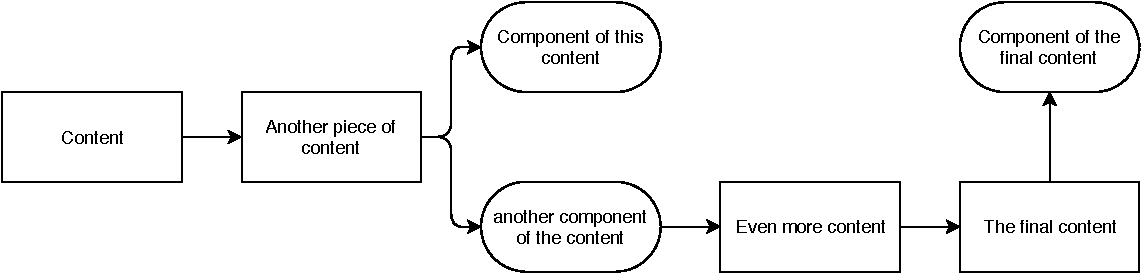
\includegraphics[width=\textwidth]{MapExample.pdf}
	\caption{An example of a concept map displaying relations between different content and components, with arrows illustrating the flow of actions.}
	\label{fig:ConceptMapExample}
\end{figure}
%
\noindent
This leads to the important matter of whether the recruited subjects should complete the task individually or in a group. For creative processes in general it isn't possible to say that one of the approaches objectively is more effective than the other, as people are different. Some think best by themselves, while doodling on a piece of paper, and others require the group setting to think more creatively \parencite[][362]{PDF:InformationArchitecture}. On the basis of this, it seems difficult to assume that one of the approaches fits better to the workshop than the other. It's therefore decided to conduct task 1 individually and task 2 as a group task, accommodating for the different type of people participating. This, however, also requires measures for making sure that the subject actively engage in this group session and don't hold back. The workshop is therefore initiated with an "ice-breaker" in order to make it more relaxed. It's assumed that by laughing together early on, they will be more keen to criticise bad ideas later on.

\section{Analysis method}
\label{AnalysisMethod}
Analysing this user study is split into two parts, as the card sort and workshop are conducted separately. It's however still the intention to unify them in the end and as such reach a single conclusion. This conclusion must answer the question stated in the previous mentioned research question for this user study. \fxnote{Indsæt research question og henvis herfra}. For the card sort there are two overall ways of approaching the analysis, exploratory and statistical. The choice of either must support the goal of the card sort, which has an exploratory approach. As such, it seems obvious to also conduct an exploratory analysis of the data, but in reality both are applicable. Should the amount of data turn out to be small, \textcite{WEB:DonnaSpencer} would recommend to just use the exploratory analysis, and in the case of much data, she recommends to start with the exploratory analysis and move to statistical, if it would provide further insight \parencite[][177]{WEB:DonnaSpencer}.

With the exploratory analysis, the goal in this analysis is to find patterns within the groupings that makes sense in correlation with studying the information architecture. More specific, this means answering questions such as:
%
\begin{itemize}
	\item What groups do the subjects form?
	\item Which cards are typically grouped together?
	\item how do they label these groups?
\end{itemize}
%
\noindent
The first step of the analysis is to gather the results in a spreadsheet in order to get a better overview of the data. The next step is then to standardise the labels. The subjects may use similar labels for their groups, and the question in these cases is, whether they actually mean the same thing. Gaining an overview of this can be tricky, as the similarity can be in either language or idea, and it therefore requires a thorough look at, not only the label name, but also at similarity in groupings. Subjects may group items together and label them differently, even though the idea may be the same \parencite[][184]{WEB:DonnaSpencer}. When choosing a standardised label name, it is then necessary to use the most prevalent labels. After this phase, the objective then is to examine the groups. This process is eased by presenting the data in a big matrix, making the groupings more clear. The potential tendencies in these groupings will then indicate whether the subjects understand the content similarly and have similar expectations \parencite[][191]{WEB:DonnaSpencer}. This process can also be supplemented by the reverse approach, looking at what is different, and as such getting a broader look at the data. The whole process may be further aided by also looking at any comments given by the subjects. As it has already been mentioned, the card sort is followed by a survey giving them a chance to elaborate on their reasoning, and these comments can therefore be investigated to provide clarifications if necessary. \\

\noindent
For the workshop, it's of interest to explore, whether the subjects have similar or different mental models for solving task 1. What content do they include in their explanations, In what order do they present this content, and which actions are required? \textcite{WEB:ConceptMapAnalysis} proposes a method for such analysis that involves combining individual mental models into a shared mental model. In this approach, a somewhat mutual consensus is required of how to construct the individual mental models. Otherwise it will be hard to make comparisons and furthermore difficult for the subjects, if they're confused of how the other subjects are completing the task. The purpose of this analysis is however not to evaluate how well the users work together but generate mental models for the information architecture. The shared mental model should be understood as the result of combining different mental models, and with the process of constructing it kept in mind, \textcite{WEB:ConceptMapAnalysis} also refers to it as an \textit{analysis constructed shared mental model (ACSMM)}.

\autoref{fig:ACSMM} illustrates simplistically how this model is constructed from the individual mental models. The first step of this process is to have the subjects communicate their individual models, which is done in the shape of concept maps (see \autoref{WorkshopApproach}). The models are then analysed in order to construct the shared model, and this analysis is done from a combination of their concept maps and the video recordings of their explanations. Their presentations are therefore coded with the intention of easing the comparison phase. The shared model is then constructed by finding the items shared by the subjects from a sharedness criterion of 50\%. This means that if the concepts, actions etc. appear more than half of the time, they are included \parencite[][128]{WEB:ConceptMapAnalysis}.
%
\begin{figure}[H]
	\centering
	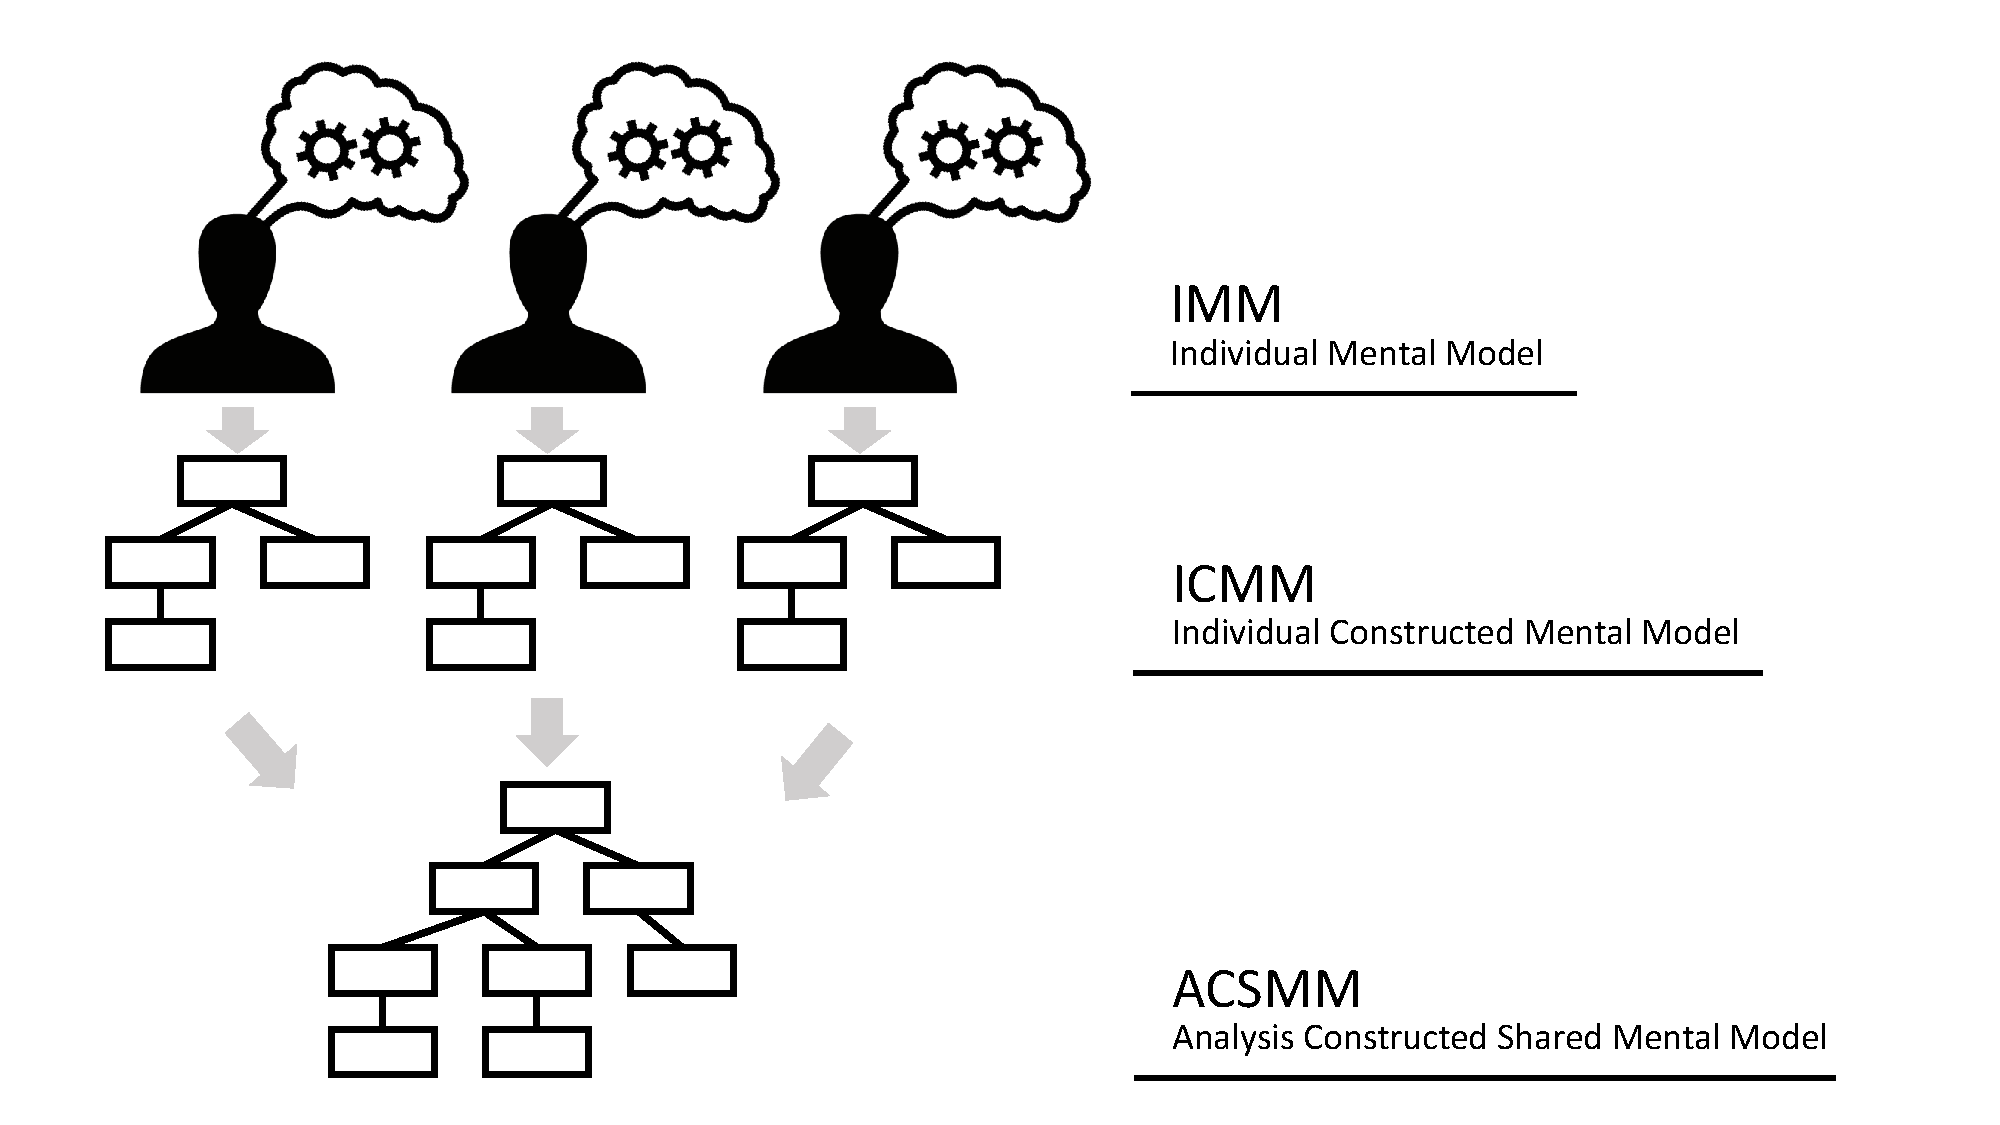
\includegraphics[width=0.95\textwidth]{ACSMM.pdf}
	\caption{The process of constructing a shared mental model from a group of individual mental models.}
	\label{fig:ACSMM}
\end{figure}
%
\noindent
The challenge with applying this method, however, lies in if the subjects produce concept maps with substantial differences. If there is no mutual consensus to how they should complete the task, they may use different approaches, making a comparison difficult. The subjects are given the same instructions to the workshop, but if their visual representations of the solutions simply take different routes, then the analysis should be approached more cautiously. The intention will nevertheless be to find common traits for the responses given in task 1, but it may not be possible to completely outline a shared mental model. For task 2, this issue is meanwhile not present, as it involves the subjects agreeing on a response. The analysis of this is therefore more straightforward, as the shared mental model is made from the session itself.

\subsection{Pilot workshop}
\label{PilotTest}
Before exploring the results of the user study, it should be noted that a pilot workshop was conducted at AAU with five subjects in order to explore whether changes should be made before conducting the actual workshop. The five subjects weren't TonePrint users but still guitarists, and as such, they were given a short introduction to the TonePrint concept before the workshop was initiated. The pilot workshop went intentionally and produced a few corrections for the introductions given to the subjects in the actual workshop. It was decided to elaborate further to the subjects what they could include in their concept maps, including further specifying the definition of content, components and actions. This also included telling the subjects that they're allowed to include drawings in their concept maps, if this will help them communicate their response.

Discussions were also had on whether to re-phrase the tasks, because the subjects in the pilot workshop had some problems with fully understanding their meaning. It was however chosen to not make changes to the phrasing, as these problems regarded their understanding of the TonePrint concept. The true workshop was set to involve end-user i.e. guitarists already familiar with the TonePrint concept, so this was expected to not be an issue with them. Another change was instead made to the presentation of the tasks. The subjects in the pilot were presented an example of how to make a concept map, but while completing it, they didn't have this visual cue. It was therefore decide to include an example of a concept map next to the tasks in the presentation.

